\documentclass{scrartcl}
\usepackage[utf8]{inputenc}
\usepackage[hidelinks]{hyperref}
\usepackage{url}
\usepackage{natbib}
\usepackage{graphicx}
\usepackage{booktabs}
\usepackage{microtype}
\usepackage{cleveref} % this must be the last package to be loaded

\hypersetup{pdftitle={Orbital: Final Project Report},pdfauthor={Aldo Visconti},pdfsubject={Reviewed implementation snapshot, 16 November 2026}}

\newcommand{\emailaddr}[1]{\href{mailto:#1}{\texttt{#1}}}

\title{\LARGE
    Final Report:\\
    Orbital
}
\subtitle{Cryptocurrency Market Data \& News Aggregation Platform: Distributed Systems Course\\
2025--2026}

\author{
    Aldo Visconti \\ \emailaddr{aldo.visconti@studio.unibo.it}
}

\date{16 November 2026}

\begin{document}

% Relaxes line-breaking so long inline \texttt{} identifiers (market-ingestor,
% postgres-market-replica, etc.) don't produce overfull hboxes running into the margin.
\sloppy

\maketitle

\noindent\textbf{Implementation snapshot.} Reviewed on 16 November 2026 against
\texttt{develop} at \texttt{e763ad4}. The fetched \texttt{main} branch at \texttt{c5e362f}
contains the same application baseline. The declared release version is 1.3.0. Implemented behavior,
recorded validation, and proposals are distinguished throughout this report.

\noindent
\textbf{Orbital} is a distributed, microservices-based platform that aggregates real-time
cryptocurrency market data and a synthetic crypto-news feed behind a single API gateway, with a Kotlin
Multiplatform client (desktop and web) on top. Application logic is decomposed into two
specialized services, \textbf{market-service} and \textbf{news-service}, fronted by a
\textbf{gateway} that proxies, caches, and rate-limits public API requests.

The project combines independently owned PostgreSQL databases, shared Redis caching and rate
limiting, a three-node Sentinel quorum, and asynchronous database standbys. These mechanisms
reduce particular failure risks; they do not guarantee uninterrupted service or zero data loss.
A standalone worker collects current prices and progressively imports checksummed Binance
archives for the same tracked coins. The client exposes historical ranges, zoom, and coverage
information while keeping Binance USDT prices separate from CoinGecko USD observations.
The backend-connected client and the public, backend-free market demo have different capabilities.

\section*{Disclaimer}

Claude Code (Anthropic) and Codex (OpenAI) assisted with code, infrastructure, security
remediation, historical imports, CI troubleshooting, and report drafting from repository evidence.
Implemented behavior, proposals, and recorded validation are identified separately. The author
remains responsible for reviewing generated material and for all technical claims.

\clearpage

\tableofcontents

\section{Concept}\label{concept}

Orbital is a set of web services (a gateway and two backend services) fronting a shared
persistence/caching layer, paired with a Kotlin Multiplatform client application (desktop and
web) that consumes them.

\paragraph{Use case.} The use case is a personal market-data and news dashboard: a user wants to
see current cryptocurrency prices, a coin's price history, and recent news, without visiting
several separate sites.

\begin{itemize}
  \item \textbf{What:} The software continuously ingests cryptocurrency prices, serves a synthetic crypto-news feed, caches
  and rate-limits access to that data at a single gateway, and presents it through a searchable,
  filterable client.
  \item \textbf{Roles:} There is currently a single anonymous application role, since there are no user
  accounts and nothing distinguishes one caller from another beyond their IP address for
  rate-limiting purposes (see \cref{security} for a proposed design that would introduce real
  roles).
  \item \textbf{Interaction:} Users interact via a desktop window or a web browser. Interaction is
  pull-based and relatively low-frequency from any single user's perspective (opening the app,
  searching for a coin, expanding its chart, switching a news category), but the client also
  auto-refreshes periodically, and many independent users may be doing this concurrently.
  \item \textbf{Data Storage:} The system does not store any user-specific data, since there is no
  concept of a user account to attach data to. The data it \emph{does} store, price snapshots and
  news articles and archive-import metadata, is global and shared across users. It is persisted
  in two separate PostgreSQL databases, one per backend service.
\end{itemize}

\paragraph{Why is distribution needed?} Distribution was deliberately chosen for the following
reasons, not imposed artificially:

\begin{itemize}
  \item \textbf{Resource Sharing:} Backend-connected clients observe shared market and news data, so it makes
  sense to fetch and store it once, centrally, rather than have every client poll CoinGecko
  independently, which would also multiply load against CoinGecko's own rate
  limits~\citep{coingecko2024api}.
  \item \textbf{Fault Tolerance:} A single unreplicated database or cache instance would make the
  whole platform's persistence path a single point of failure; \cref{fault-tolerance} describes
  how this is addressed.
  \item \textbf{Independent Scalability:} The gateway is the component every backend-connected client talks to,
  so it is the one component that needs to be horizontally scalable independently of the two
  backend services behind it; \cref{availability} describes how this was designed for.
  \item \textbf{Educational Purpose:} To implement and analyze real distributed-systems patterns,
  namely streaming database replication, quorum-based cache failover, a distributed rate limiter,
  and CAP-theorem trade-offs, in a project small enough to reason about end to end.
\end{itemize}

\section{Requirements Elicitation and Analysis}\label{requirements}

\subsection{Functional Requirements}\label{functional-requirements}

\begin{description}
  \item[FR1] The connected application shall provide current USD market data for the existing
  top-20 selection by market capitalization. \\
  \emph{Acceptance:} \path|/api/v1/market/prices| returns a success envelope containing the
  selected coins, prices, market caps, volumes, changes, and observation timestamps.

  \item[FR2] The system shall provide source-labelled historical prices for a tracked coin,
  including available Binance pair history and a separately retained CoinGecko USD series. \\
  \emph{Acceptance:} \path|/api/v1/market/history-range/{coinId}| returns ascending timestamped
  samples, source and quote, selected bounds, resolution, loaded coverage, gaps, and import state.
  The legacy price-array and timestamped-history endpoints remain available.

  \item[FR3] The system shall expose a clearly identified synthetic crypto-news feed with
  category validation. \\
  \emph{Acceptance:} the default and CRYPTO categories return synthetic articles; other supported
  categories return no articles, and an unknown category is rejected with HTTP 400. Real NewsAPI
  integration is outside the implemented scope.

  \item[FR4] The system shall expose previously persisted news independently of an external
  provider. \\
  \emph{Acceptance:} \path|/api/v1/news/history| returns stored articles in descending publication
  order, optionally filtered by category. Repeated storage of the same article is idempotent.

  \item[FR5] The client shall support labelled market/news search, news category filters, empty
  results, and refresh recovery. \\
  \emph{Acceptance:} filtering updates the visible list; a failed refresh preserves previous
  content with a stale-data notice and retry control rather than presenting it as newly fetched.

  \item[FR6] The connected client shall expose 24H, 7D, 1M, 1Y, and All available chart ranges,
  request finer detail for narrower windows, and make incomplete coverage visible. \\
  \emph{Acceptance:} range/source selection or zoom issues a new history request; obsolete requests
  cancel, gaps are not connected by the price line, and earliest/latest loaded dates are shown.
  The backend-free public demo retains a seven-day relative overview.

  \item[FR7] Current-price collection and historical imports shall continue independently of
  client traffic for the same tracked universe. \\
  \emph{Acceptance:} the default snapshot interval is 15 minutes; archive jobs and imported-file
  checksums persist in PostgreSQL, survive restarts, and stop being scheduled for inactive coins.
  Coverage grows progressively; complete history is not promised immediately after first startup.
\end{description}

\subsection{Non-functional Requirements}\label{non-functional-requirements}

\begin{description}
  \item[NFR1 (Availability)] A cache or rate-limit backend failure shall not automatically reject
  an otherwise serviceable request. \\
  \emph{Acceptance:} cache failures attempt the upstream request and Redis rate-limit failures
  allow the request. A valid cache hit can avoid an upstream call; cache expiry or simultaneous
  upstream failure can still produce an error. This is a bounded availability policy, not an SLA.

  \item[NFR2 (Recovery)] Each PostgreSQL primary shall have an asynchronous standby and persistent
  storage to support recovery. \\
  \emph{Acceptance:} a recorded replication check shows streaming and matching WAL positions.
  Unreplicated transactions can be lost on primary failure; promotion and service reconnection
  remain manual. Matching positions at one instant do not prove zero-loss failover.

  \item[NFR3 (Scalability)] Gateway replicas shall share one Redis-backed budget per client. \\
  \emph{Acceptance:} tests cover client identity, quota exhaustion, and fail-open behavior;
  forwarded identity is trusted only behind the private nginx ingress. Sustained concurrent
  multi-replica load remains an evaluation task.

  \item[NFR4 (Resource Bounds)] Repeated cacheable reads shall avoid redundant upstream calls;
  historical responses and imports shall remain bounded. \\
  \emph{Acceptance:} repeated identical cacheable requests share the short-TTL response. Range
  queries sample the whole selected span at a bounded resolution; network/ZIP size limits and
  small background batches bound archive work. Range endpoints are not gateway-cached.

  \item[NFR5 (Observability)] Liveness, readiness, and metrics shall expose different operational
  information without consuming the public request budget. \\
  \emph{Acceptance:} \path|/health| remains a liveness check, \path|/ready| reports required
  dependency availability, and \path|/metrics| supplies Prometheus metrics. Grafana is optional
  through the admin Compose profile.

  \item[NFR6 (Integrity and Safety)] Invalid persistence batches shall roll back, provider
  identities and currencies shall remain explicit, and errors shall not expose internal details. \\
  \emph{Acceptance:} real-PostgreSQL tests cover atomic failure and deduplication; Binance downloads
  require matching SHA-256 checksums; source/quote metadata and safe error envelopes are returned.
\end{description}

\subsection{Implementation Choices}\label{implementation-choices}

\begin{enumerate}
  \item \textbf{Technical Stack:} Application logic across backend, client, and shared library
  modules is written in Kotlin, with Ktor~\citep{ktor2024docs} as the backend HTTP
  server/client framework.
  %
  \begin{itemize}
    \item \emph{Justification:} Ktor's coroutine-based concurrency model suits the I/O-bound
    proxy/aggregation workload of a gateway and two backend services well, and keeping the whole
    backend on one language and build toolchain removes a language boundary that would otherwise
    need to be crossed for no architectural reason.
  \end{itemize}

  \item \textbf{Client Platform:} Kotlin Multiplatform with Compose Multiplatform, targeting both
  JVM desktop and \texttt{wasmJs} web from a single codebase.
  %
  \begin{itemize}
    \item \emph{Justification:} avoids maintaining two separate UI codebases for what is
    otherwise the same client logic, and keeps the client in the same language as the backend.
  \end{itemize}

  \item \textbf{Database:} PostgreSQL 15~\citep{postgresql2024docs}, accessed through Exposed
  and parameterized JDBC queries, with one independent database per backend service (\texttt{market\_data},
  \texttt{news\_data}).
  %
  \begin{itemize}
    \item \emph{Justification:} a mature, well-understood relational engine with first-class
    streaming replication, directly relevant to NFR2. Separate databases per service keep each
    service's persistence failure domain isolated from the other's.
  \end{itemize}

  \item \textbf{Cache and Coordination:} Redis, accessed via Jedis, behind either a plain
  \texttt{JedisPool} or a Sentinel-aware \texttt{JedisSentinelPool}~\citep{redis2024sentinel}
  depending on configuration.
  %
  \begin{itemize}
    \item \emph{Justification:} Redis is the de facto standard for this kind of short-TTL proxy
    cache, and Sentinel is its own built-in high-availability mechanism rather than a
    third-party add-on, keeping the operational surface small.
  \end{itemize}

  \item \textbf{Load Balancing:} nginx, in front of however many gateway replicas are running.
  %
  \begin{itemize}
    \item \emph{Justification:} a minimal, well-understood reverse proxy was sufficient; nothing
    in this project's requirements called for a full service mesh.
  \end{itemize}

  \item \textbf{Deployment:} Docker Compose~\citep{docker2024compose} orchestrating the entire
  stack on a single host.
  %
  \begin{itemize}
    \item \emph{Justification:} reproducibility across development and this report's own manual
    verification work (\cref{acceptance-test}), without the operational overhead of a
    multi-host orchestrator that this project's scale does not need.
  \end{itemize}
\end{enumerate}

\subsection{Relevant Distributed System Features}\label{ds-features}

\paragraph{Transparency.} The backend-connected \texttt{orbital-app} talks
to the gateway (\cref{architecture}); it has no knowledge of there being two backend services,
two PostgreSQL primaries, a Redis Sentinel quorum, or (potentially) several gateway replicas
behind a load balancer. Provider identity, quote currency, gaps, and incomplete imports are
intentionally visible to users. The separate public demo calls CoinGecko directly.

\paragraph{Fault tolerance, dependability.} Highly relevant, and the area with the most concrete
work in this project: PostgreSQL streaming replication for both databases, a Redis Sentinel
quorum, retry-with-backoff on startup, and fail-open behaviour in both the cache and the rate
limiter. Uninterrupted service is not strictly required (this is not a payments system), but
losing previously-collected price/news history to a single container crash was judged
unacceptable given FR2/FR4's whole point is to keep that history around. \Cref{fault-tolerance}
details how.

\paragraph{Scalability.} Relevant specifically at the gateway, the entry point for backend-connected
client requests; not particularly relevant at the two backend services, which
are not designed to need more than one replica each. \Cref{availability} covers the design;
\cref{future-works} is explicit about what has and has not actually been exercised under load.

\paragraph{Security, trust.} Public HTTP reads remain anonymous; account authentication and
role-based authorization have not been implemented. Existing controls nevertheless address
concrete risks: loopback-only development exposure, a trusted private proxy boundary, safe errors,
deadlines, bounded imports, non-root runtime users, dependency checks, and careful source mapping.
Database credentials and IP-based operational identifiers still require protection even without
user accounts. A proposed identity extension is separated from these controls in \cref{security}.

\paragraph{Resource sharing.} Central to the system's existence (\cref{concept}): price and news
backend observations and imported archive files are retained centrally, while short-TTL
caches reduce repeated live requests. The backend-free demo is an explicit exception; the Redis cache, the Redis-backed rate-limit counters, and both PostgreSQL
databases are all resources shared across however many gateway/service replicas are running.

\paragraph{Openness, interoperability.} Relevant at the boundaries: the backend talks to
CoinGecko's public REST/JSON API and Binance's HTTPS archive as external systems, and the client
and backend communicate over plain HTTP/JSON rather than a project-specific binary protocol, so
either side could in principle be replaced independently as long as that contract holds.

\paragraph{Evolvability, maintainability.} Actively designed for: the backend is split into
independently buildable Gradle modules, dependency versions are centralized, and pushes/PRs targeting main or develop run
automated tests, static analysis (detekt), and formatting checks (ktfmt/spotless) in CI, with
releases cut automatically from Conventional Commit history. This matters because the project
has already gone through several rounds of adding infrastructure (replication, Sentinel, a
distributed rate limiter) without a rewrite.

\paragraph{Performance, concurrency.} Relevant but not under strict quantitative targets: there
is no SLA on response time. Ktor's coroutine-based I/O and the proxy cache (\cref{availability})
keep the gateway from doing redundant work, which matters more for not wasting CoinGecko's own
rate-limited quota than for raw latency.

\paragraph{Economy, costs.} A real, concrete driver of at least one implementation decision
already made: news-service serves synthetic articles without unused external requests. Binance
archives avoid a paid full-history API dependency, while CoinGecko public-plan requests are
bounded. Free access still carries coverage, quota, storage, and dataset-license constraints.

\section{Design}\label{design}

This chapter explains the strategies used to meet the requirements identified in
\cref{requirements}, motivated against the features identified in \cref{ds-features}.

\subsection{Architecture}\label{architecture}

Orbital uses a \textbf{Microservices} architecture decomposed along functional boundaries. After
analysis, three macro concerns were identified:

\begin{itemize}
  \item \textbf{Market Data Logic:} Performed by \texttt{market-service} and the standalone
  \texttt{market-ingestor} worker. Combines current CoinGecko prices with a resumable Binance
  archive importer. The API reads observations and can update tracking metadata/enqueue import
  requests; only the worker collects market observations. The worker exposes no HTTP endpoint.
  \item \textbf{News Logic:} Performed by \texttt{news-service}. Handles the (currently mocked)
  news feed and its own persisted archive. Exposes a REST API.
  \item \textbf{Edge:} Handled by \texttt{gateway} (the single client-facing entry point, caching
  and rate limiting) and \texttt{gateway-lb} (the load balancer in front of however many gateway
  replicas are running).
\end{itemize}

This \textbf{functional decomposition} ensures that market-service and news-service, two
independent functional domains with separate persistence failure modes, can evolve, be deployed, and
fail independently of one another, and that the one component actually needing to scale (the
gateway) is not coupled to the two that do not. The client, \texttt{orbital-app}, is
architecturally a classic thin client: all domain logic and persistence live behind the gateway,
and the client's own role is presentation and local UI state only.

\subsection{Infrastructure}\label{infrastructure}

The infrastructure contains the following components. Backend containers are orchestrated by
one \texttt{docker-compose.yml}; desktop and browser clients run separately:

\begin{itemize}
  \item \textbf{Client-side:} \texttt{orbital-app}, a Compose Multiplatform application (desktop
  JVM and \texttt{wasmJs} web). The full client uses the gateway; the separate public demo calls
  CoinGecko directly and has neither server-side archives nor a news tab.
  \item \textbf{Edge Layer:} \texttt{gateway-lb}, an nginx instance acting as a reverse proxy. It
  provides a single entry point on port \texttt{8080}, hides however many \texttt{gateway}
  replicas sit behind it. A variable upstream and Docker DNS resolver with a short cache allow
  renewed discovery instead of a single address fixed when nginx starts.
  \item \textbf{Service Layer:} \texttt{gateway} (routing, caching, rate limiting),
  \texttt{market-service} and \texttt{news-service} (independent Ktor applications, each owning
  its own database), and \texttt{market-ingestor} (a worker process with no HTTP interface).
  \item \textbf{Persistence Layer:} Two independent PostgreSQL 15 primaries:
  \texttt{postgres-market} (owned by market-service/market-ingestor) and \texttt{postgres-news}
  (owned by news-service), each with its own streaming-replication standby.
  \item \textbf{Cache / Coordination Layer:} A Redis primary and replica, monitored by a
  three-node Sentinel quorum.
  \item \textbf{Monitoring:} Prometheus scrapes all three HTTP services. Grafana is provisioned
  but starts only with the optional \texttt{admin} profile.
  \item \textbf{Administration:} pgAdmin is also gated by the \texttt{admin} profile.
\end{itemize}

\begin{figure}
\centering
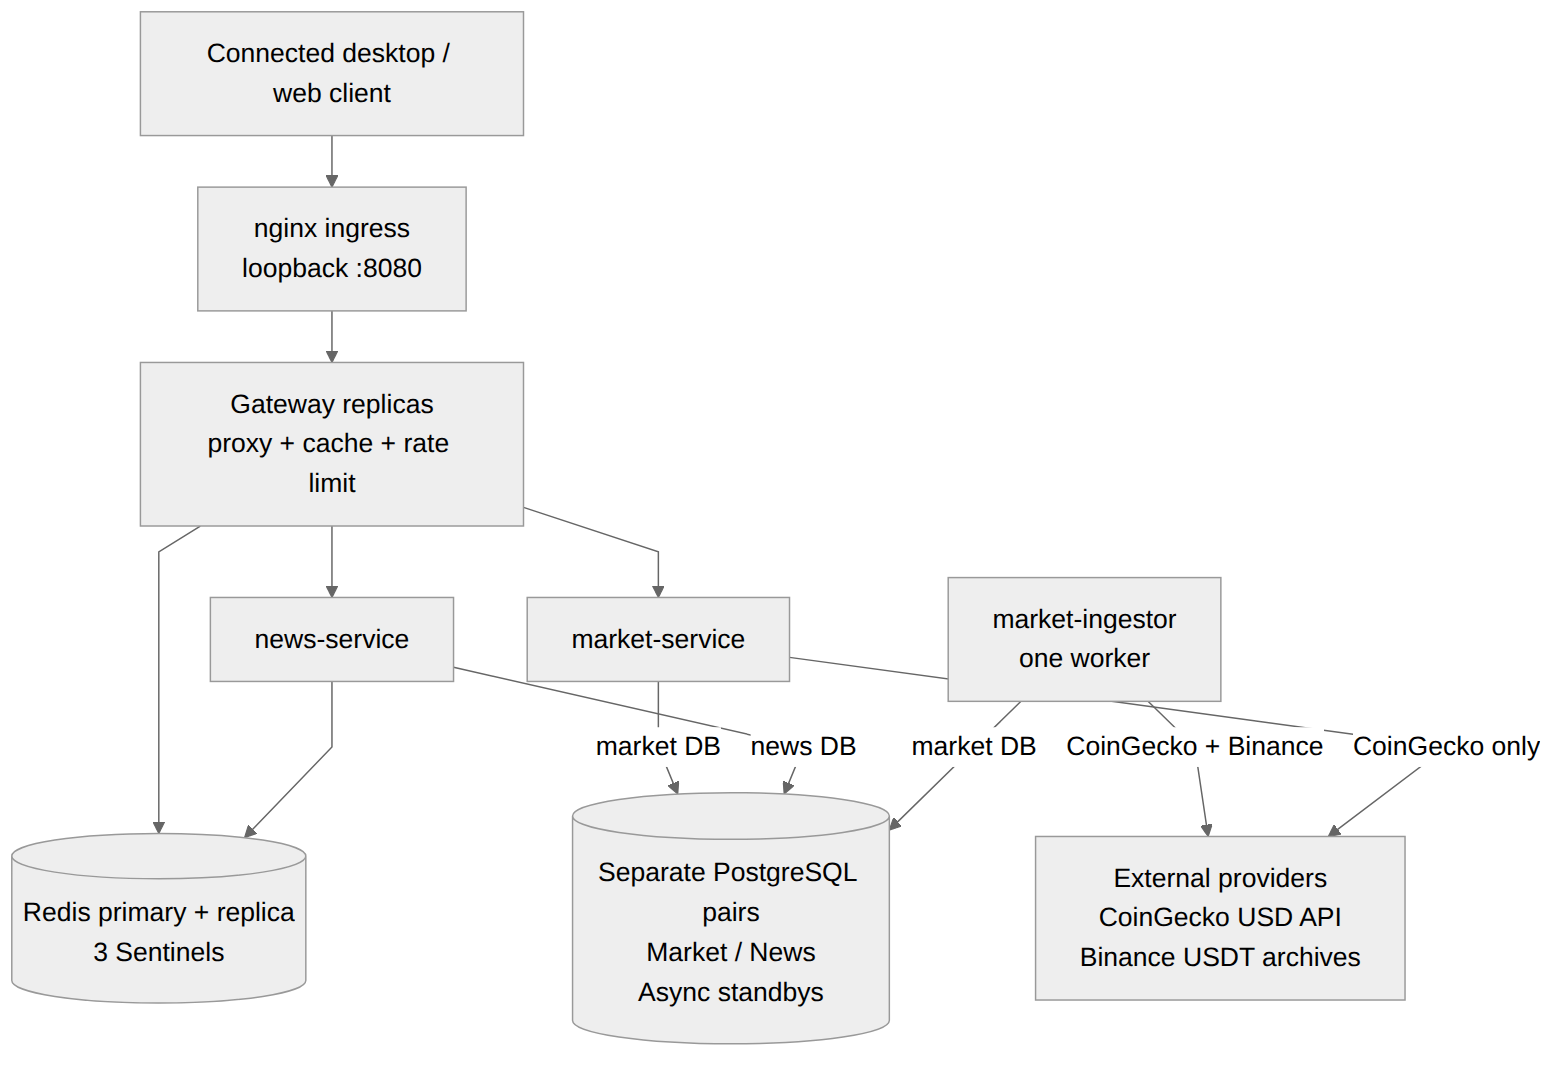
\includegraphics[width=0.9\textwidth]{figures/infrastructure.png}
\caption{Core data paths across the client, edge, services, providers, and persistence layers.
Monitoring and optional administration components are described in the text.}
\label{fig:infrastructure}
\end{figure}

Backend containers currently run on a single host, on one Docker bridge network
(\texttt{orbital-net}); nothing in the design assumes same-host placement, but nothing in the
current deployment spans more than one host either. Client applications run outside that
container network; Binance and CoinGecko are external providers. That would be the natural next step if
Orbital needed genuine geographic distribution, which \cref{concept} does not identify as a
driver for this product.

Components find each other by \textbf{name}, not by hardcoded IP address: Docker Compose's
embedded DNS resolves each service's name (e.g.\ \texttt{postgres-market}, \texttt{redis},
\texttt{redis-sentinel-1}) to whichever container is currently running it. For Redis specifically,
this is deliberately \emph{not} enough on its own: a client that resolved \texttt{redis} once and
cached the connection would keep talking to the old master after a Sentinel failover. Both the
gateway and news-service therefore talk to Redis through the Sentinel quorum
(\path|REDIS_SENTINEL_HOSTS|) rather than a fixed hostname, asking the quorum who the current
master is. Sentinel runtime files are writable in separate persistent volumes, seeded with a
numeric monitor address so a stopped Docker hostname cannot block failover. This makes the infrastructure \textbf{location-transparent} in
the sense relevant to \cref{ds-features}: nothing downstream of the gateway needs to know which
physical Redis node is currently serving as master.

\subsection{Modelling}\label{modelling}

\subsubsection{Domain Entities}\label{modelling-entities}

Each service owns its persistence schema; domain records are not shared across service databases.
Market persistence includes the following records:

\begin{itemize}
  \item \textbf{USD observations:} \path|market_prices| stores the CoinGecko coin ID, display
  metadata, USD market values, Unix-second observation time, and expected sampling interval.
  Deterministic IDs and a coin/time check skip repeated observations while retaining older rows.
  \item \textbf{Binance candles:} \path|history_candles| stores coin ID, verified USDT pair,
  closing timestamp, closing price, and interval. IDs distinguish pair, interval, and time.
  \item \textbf{Tracked coins:} \path|history_coins| records active membership, display metadata,
  verified pair, and the last identity-lookup time. Only the existing top-20 selection is active;
  discovering Binance files does not add assets. Stored data survives a coin leaving the list.
  \item \textbf{Import jobs:} \path|history_jobs| stores source, normalized time window,
  resolution, priority, state, and retry timing. User-selected windows receive higher priority.
  \item \textbf{Imported files:} \path|history_files| records archive path and checksum in the
  same transaction as the imported candles. The older \path|market_backfills| marker table remains
  for compatibility; the archive workflow uses durable jobs and the file ledger instead.
\end{itemize}

News persistence stores article metadata and category in the news database. Stable IDs derived
from article URL and category prevent repeated feed requests from duplicating an article. These
records are a retained archive, not a separate observation row for every read.

\begin{figure}[tbp]
\centering
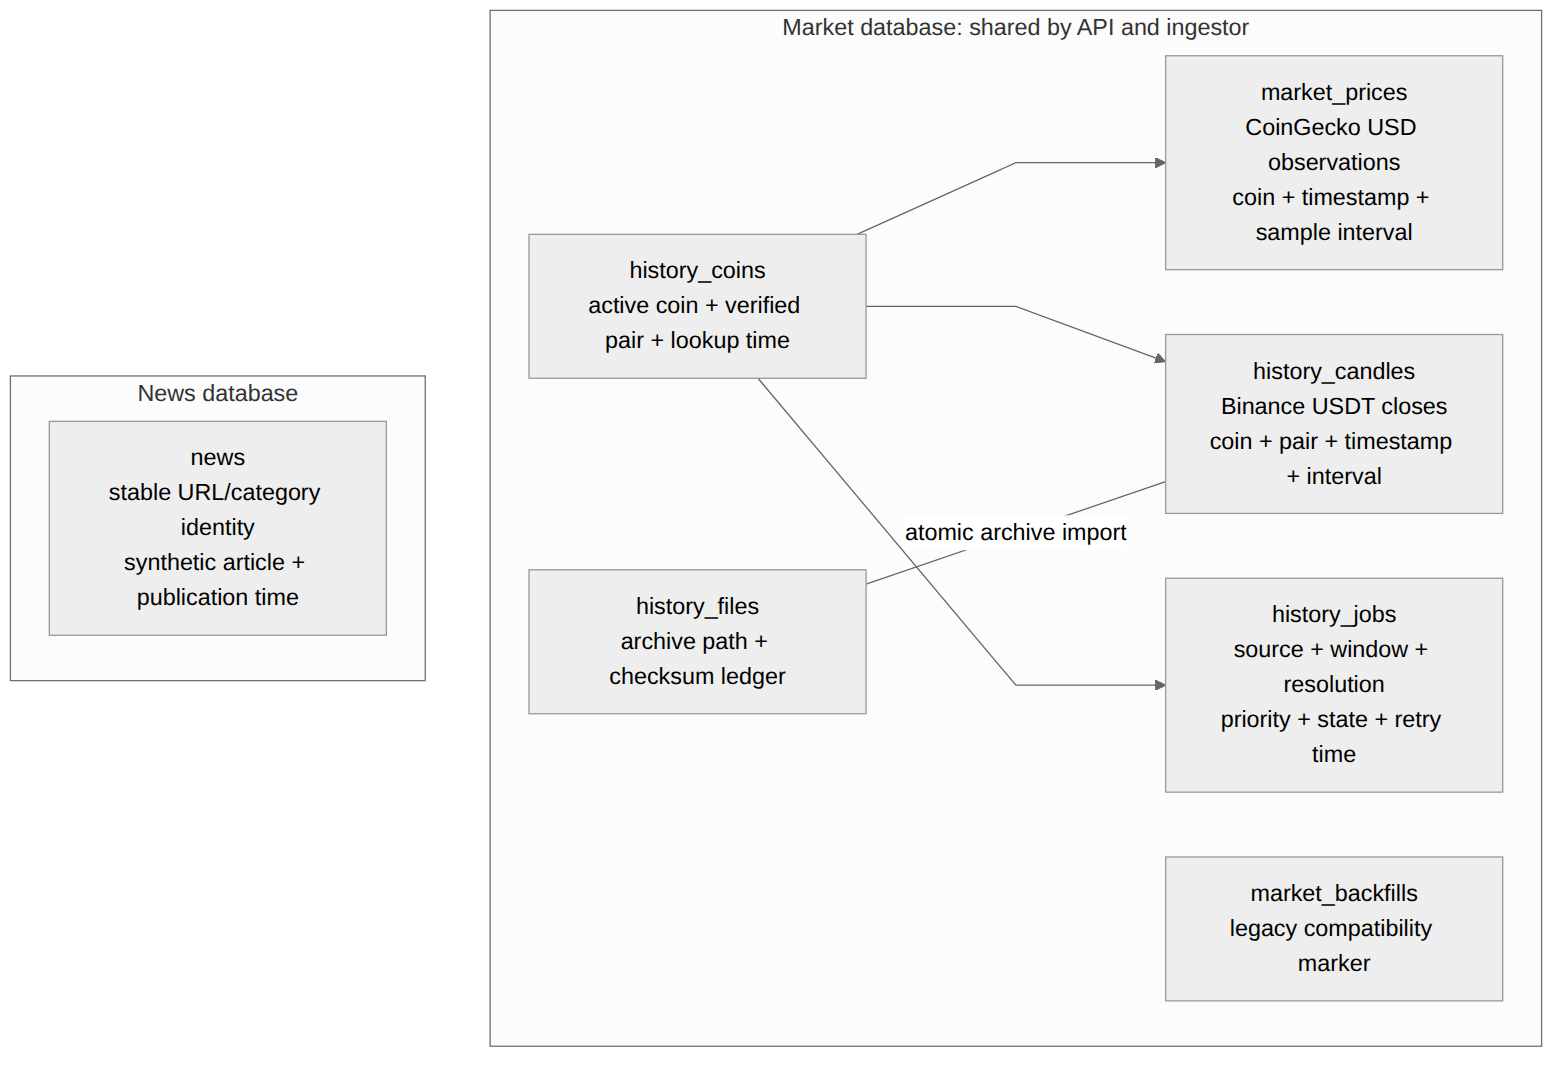
\includegraphics[width=0.98\textwidth]{figures/domain-entities.png}
\caption{Logical market records, durable archive state, and the independent news archive.
Arrows show associations rather than physical foreign-key constraints.}
\label{fig:domain-entities}
\end{figure}

\subsubsection{Resumable Historical Imports}\label{modelling-backfill-gate}

A single \texttt{hasHistory(coinId)} check cannot distinguish one live observation from a
complete historical import. The worker therefore uses durable jobs and per-file completion,
rather than treating the existence of any price as proof that backfill is finished.

On each collection cycle, the worker refreshes the same tracked selection and saves current USD
snapshots. It schedules daily Binance history for verified pairs and a separate bounded
CoinGecko history request. A background coroutine imports a small batch, commits candle data and
its checksum ledger atomically, and yields to other work. A failed provider receives a retry delay;
database interruptions do not terminate the queue loop. Pending work for inactive coins is skipped.
The design assumes one ingestor; it does not implement distributed job leasing or exactly-once
execution across multiple workers.

Binance discovery uses paginated monthly listings and daily archives for uncovered periods.
Daily candles give long-range coverage; viewed windows request hourly or five-minute archives.
Files are SHA-256 checked, read from bounded ZIP streams without filesystem extraction, and parsed
using closing price and closing time. Binance timestamps switch from milliseconds to microseconds
in January 2025, so both formats are normalized to Unix seconds~\citep{binance2026data}.
Missing or rejected files remain incomplete work rather than silently fabricated data.

\begin{figure}[tbp]
\centering
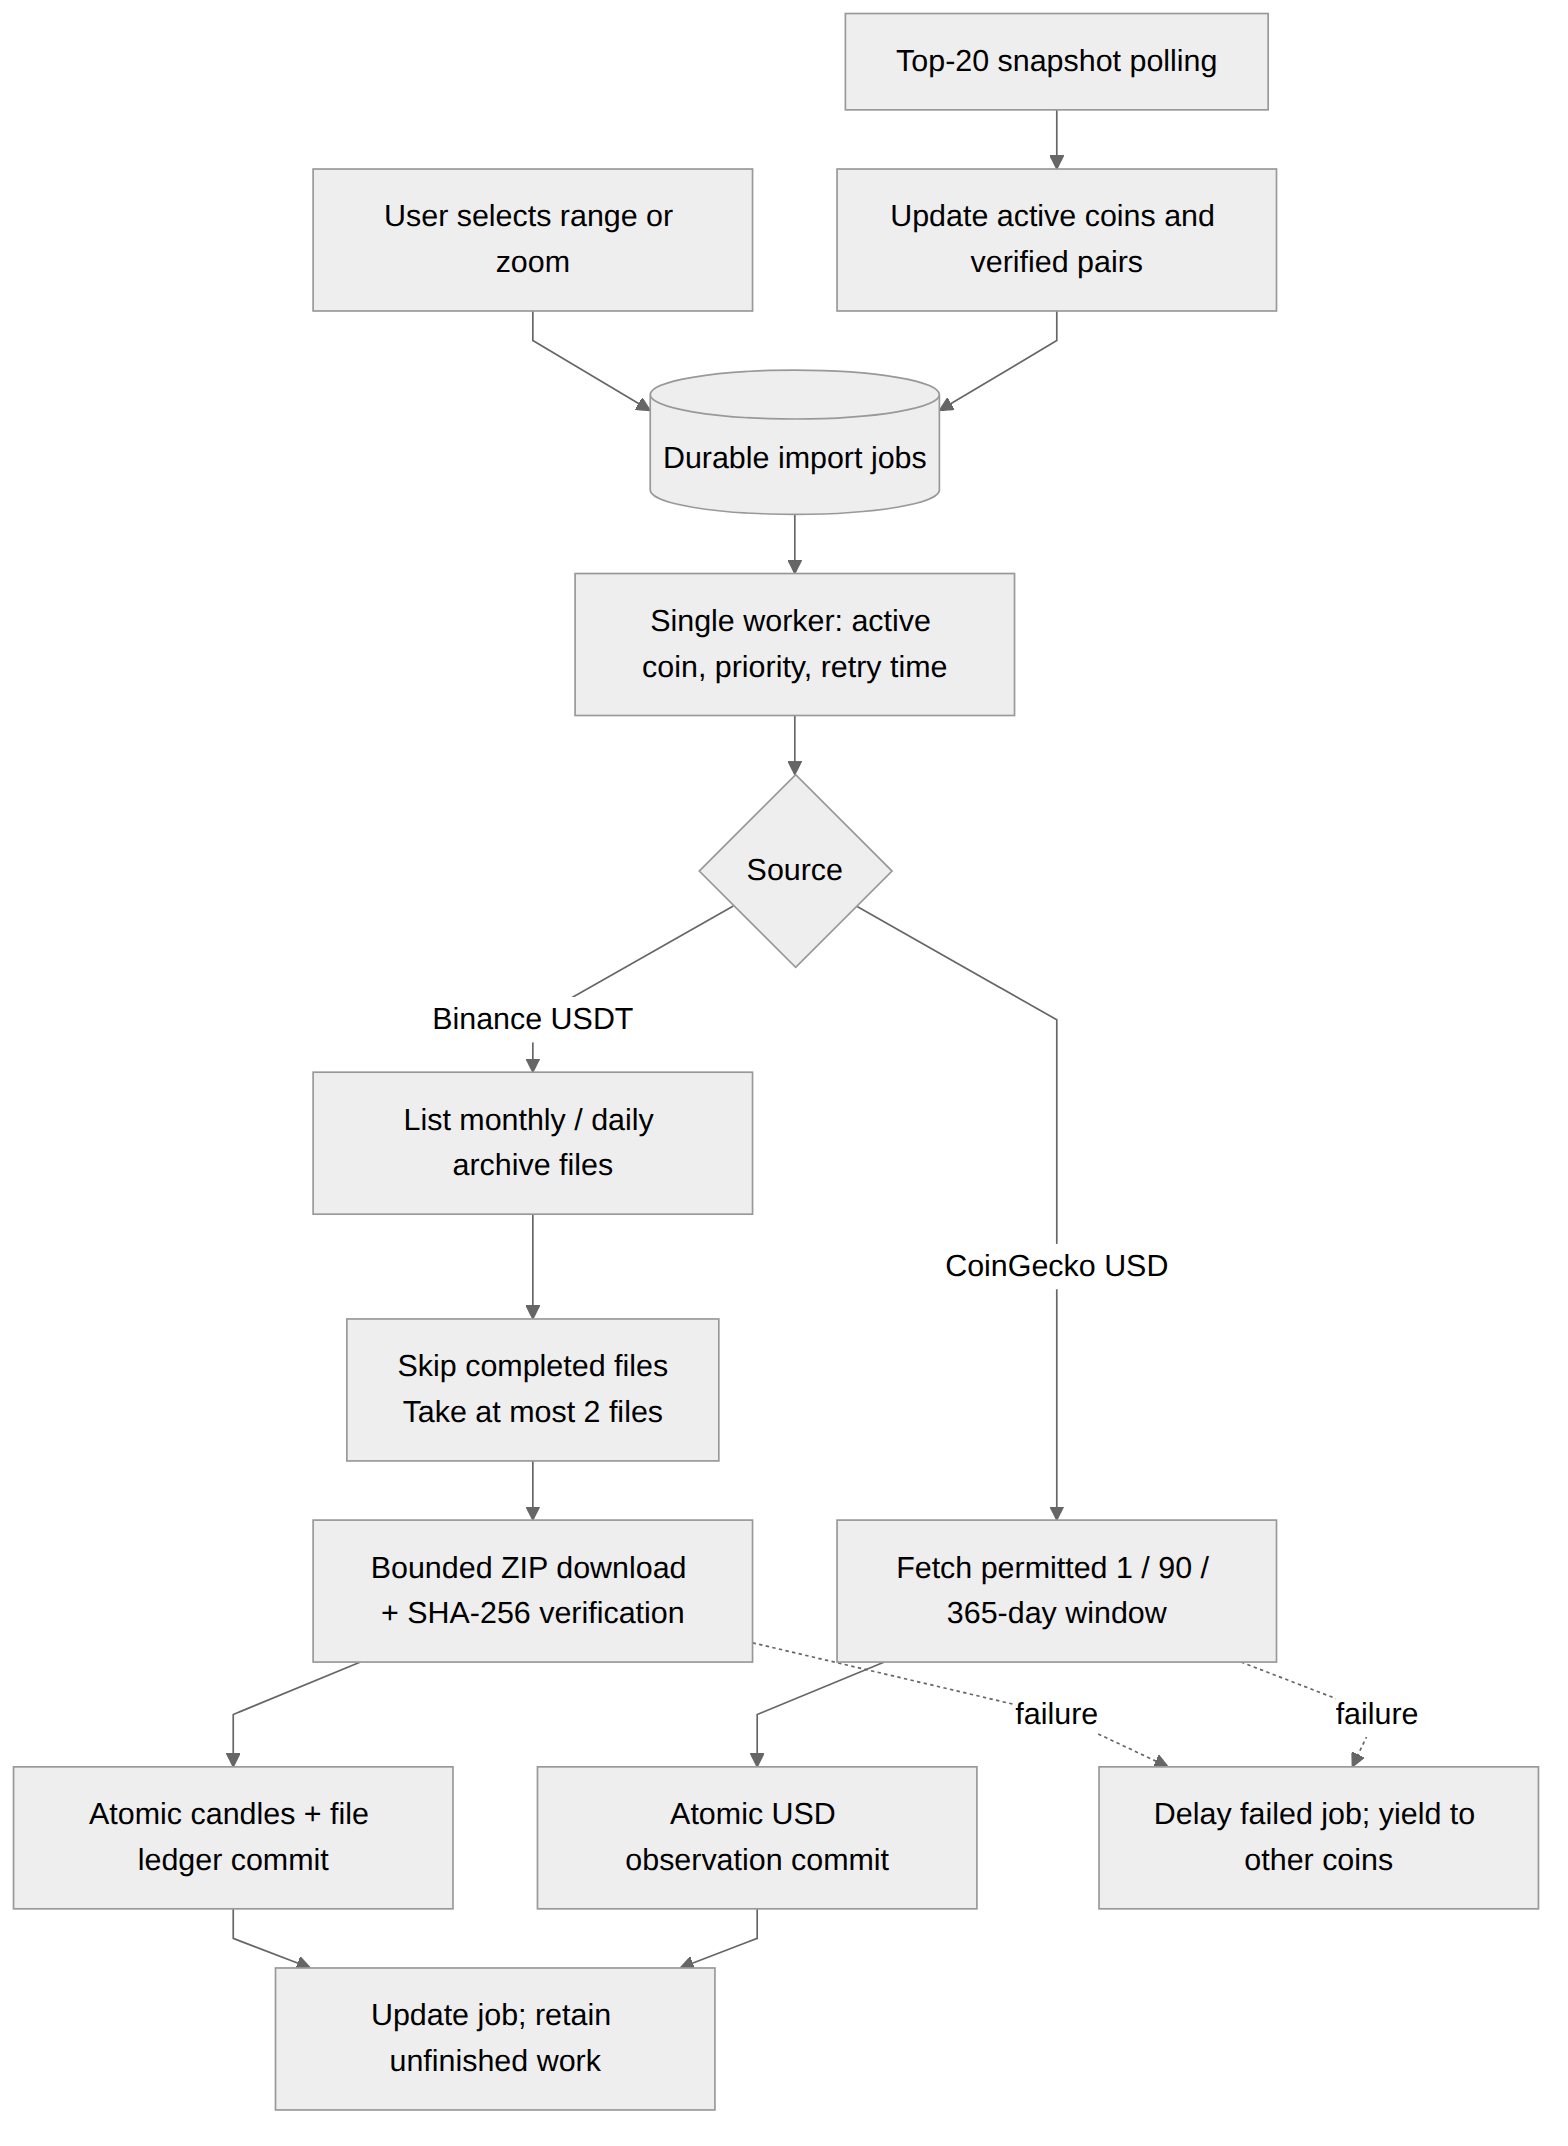
\includegraphics[width=0.94\textwidth]{figures/backfill-gate.png}
\caption{Durable job selection, checksum validation, atomic persistence, and retry behavior.}
\label{fig:backfill-gate}
\end{figure}

\subsubsection{Sources, Quotes, and Coverage}\label{modelling-coverage}

Binance series are closing prices for an explicitly identified USDT pair. CoinGecko provides
aggregated USD observations. They are selectable series, not a single spliced price history;
USDT and USD are not treated as interchangeable quote currencies. Pair mappings use explicit
coin IDs or identity-checked tickers to avoid symbol collisions. Unlisted or unverified coins use
available CoinGecko coverage, and unsuccessful identity lookups are bounded to once a day.

The public CoinGecko historical request is limited to the permitted 365-day window; stored local
observations can grow beyond that window over time~\citep{coingecko2026history}. Binance can extend
coverage back to an available pair listing, not to a coin's creation date or to periods that the
exchange never archived. Published archive files also lag the live market. No provider guarantees
that every requested interval is present.

The range API returns a \texttt{HistorySeries} containing source, quote, optional pair, timestamped
samples, requested bounds, resolution, earliest/latest loaded timestamps, detected gaps, notices,
and import state. SQL window functions select representative samples across the whole span at a
bounded resolution, rather than discarding everything before the latest 500 rows. Gaps are detected
at the displayed resolution using expected cadence; smaller missing intervals may be hidden by
coarse sampling. Earliest coverage is explicitly labelled as loaded so far while imports continue.

Binance Vision dataset terms include attribution, non-commercial use, and share-alike conditions;
the UI displays attribution and the dataset license, separately from the application code's
license~\citep{binance2026terms}. Free downloading is not a claim of unrestricted reuse.

\subsection{Interaction}\label{interaction}

User-facing API interaction is HTTP request/response. Current-price requests can be served from
a short-TTL gateway cache or forwarded to market-service, which fetches CoinGecko prices without
writing market observations. News-service serves synthetic articles, uses its own cache namespace,
and can persist them independently. The public demo bypasses the gateway and calls CoinGecko.

Historical range requests read stored observations and enqueue missing work. They do not download
ZIP files inside the HTTP handler. The worker later polls PostgreSQL for jobs and contacts the
providers independently of the requesting client. The UI polls while imports are incomplete;
there is no server-initiated push, message broker, or external streaming protocol.

\begin{figure}
\centering
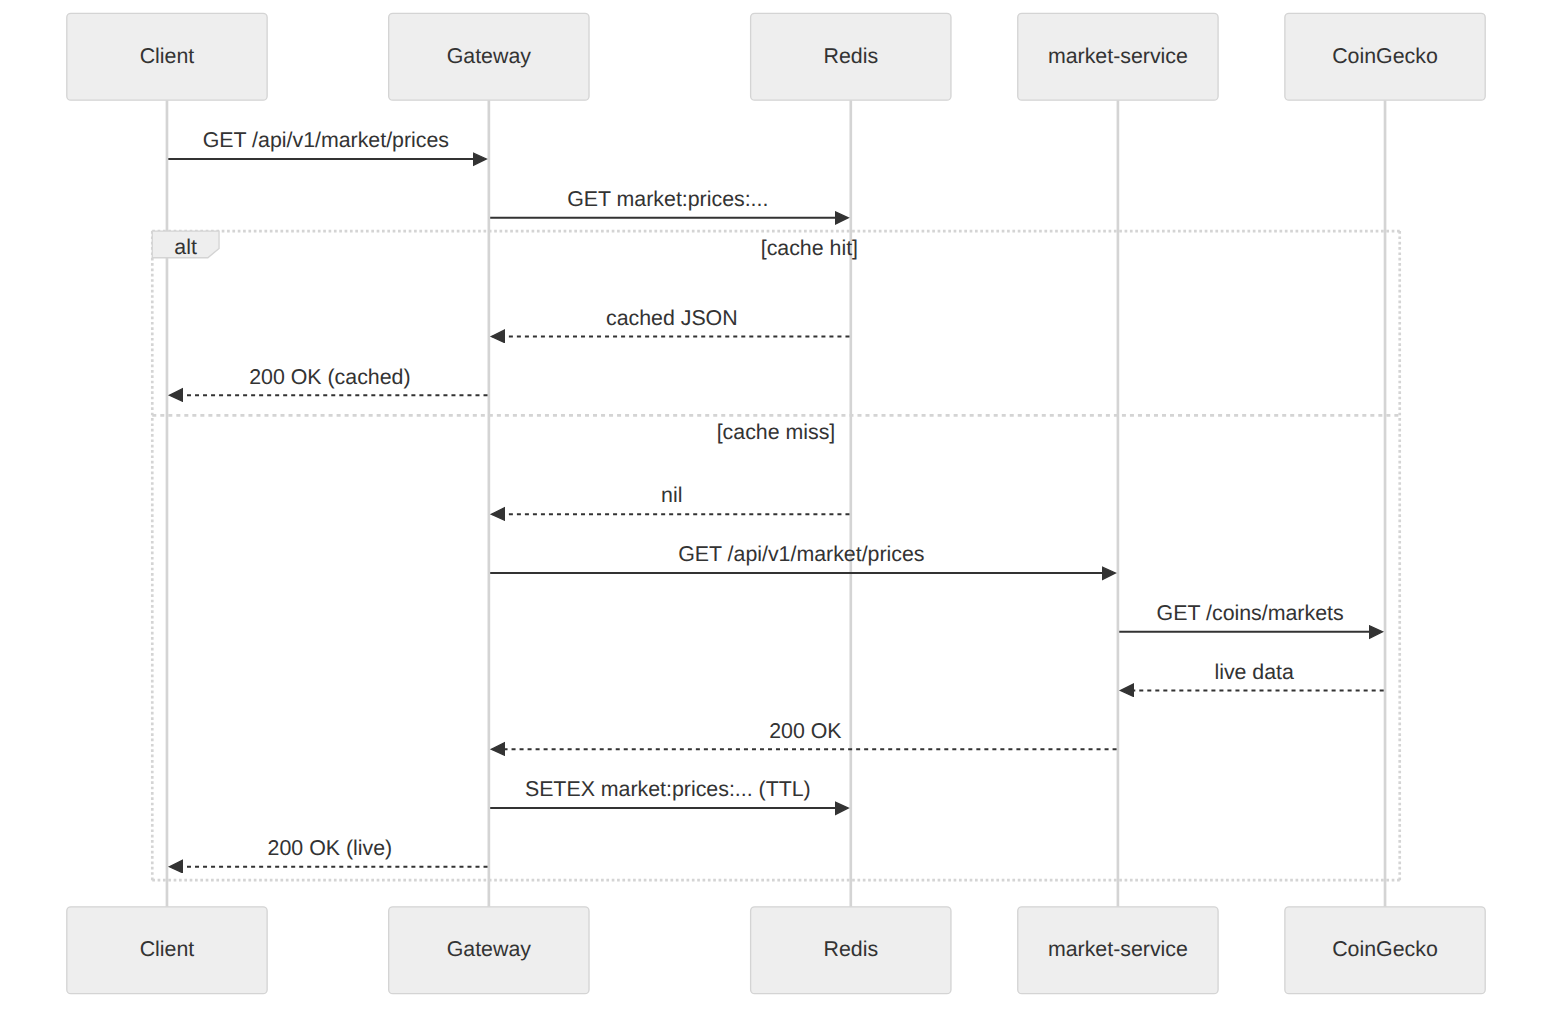
\includegraphics[width=0.85\textwidth]{figures/cache-sequence.png}
\caption{A cached vs.\ uncached \texttt{GET /api/v1/market/prices} request.}
\label{fig:cache-sequence}
\end{figure}

\subsection{Behaviour}\label{behaviour}

Shared production state lives in PostgreSQL and Redis. Gateway replicas share Redis cache
entries and client budgets; the bounded in-process fallback is intended for standalone development
and does not supply a cluster-wide quota. HTTP clients, Redis pools, and database pools have
explicit lifecycle cleanup, and blocking cache/database work is dispatched away from request threads.

The ingestor owns one collection loop and one background import loop. Durable queue state survives
its process; only one ingestor should run because job ownership is not coordinated across workers.
Repeated observations and imported files are deduplicated, but duplicate external requests from
multiple workers would still waste quotas and can race at database constraints. Market API reads
may update tracking metadata and enqueue jobs; they do not persist new price observations.
News reads may schedule best-effort storage of the synthetic feed.

\subsection{Data and Consistency Issues}\label{data-and-consistency-issues}

\subsubsection{CAP Theorem Position}\label{cap-theorem-position}

The design favors usable read responses when a valid short-TTL cache entry exists, and treats
Redis rate-limit availability as non-critical. This is an application policy motivated by the
CAP trade-off~\citep{brewer2000towards,gilbert2002brewer}; it is not a proof that the entire
multi-component deployment is a formally available AP system. An unavailable PostgreSQL primary,
an expired cache entry combined with an upstream outage, or a lost Sentinel majority can still
make operations fail. HTTP deadlines and safe error envelopes bound and describe those failures.

PostgreSQL writes remain transactional. Asynchronous standbys reduce write coupling but can lag;
promotion can lose transactions not yet received by the standby~\citep{postgresql2024docs}. Redis
replication is also asynchronous, so failover may lose recent cache entries or quota increments.
A stronger consistency or zero-loss guarantee would need a different replication and failover
configuration and corresponding tests.

\subsubsection{Consistency Model}\label{consistency-model}

Market observations retain new coin/time values, while deterministic IDs skip repeats. News IDs
are stable per URL/category. Archive candle IDs include coin, pair, interval, and timestamp;
monthly/daily overlap does not intentionally duplicate those candles. Preexisting historical
rows are preserved rather than destructively migrated.

Both repository batch saves are atomic: an invalid row is logged and the exception propagates so
the transaction rolls back. Archive file completion is committed with its candle batch. Client
responses never imply an incomplete archive import is fully covered. A cache response represents
its own short validity window and can lag provider updates; it does not supply a global snapshot
across market, news, and archive state.

\subsubsection{Shared Data and Synchronization}\label{shared-data-sync}

Market and news databases have independent schemas and pools. Import jobs and tracked-coin
metadata are mutable coordination state inside the market database, so describing all storage as
an append-only log would be inaccurate. A normalized job key coalesces repeated requests for the
same source/window/resolution. Redis atomic counter operations provide the shared per-client
rate-limit decision; this coordination is distinct from database import transactions.
The single-worker assumption limits import concurrency without claiming distributed leasing.

\subsection{Fault-Tolerance}\label{fault-tolerance}

\subsubsection{Service Isolation via Independent Databases}\label{fault-tolerance-isolation}

Because market-service and news-service are independent processes with independent databases and
independent HikariCP connection pools, the failure or overload of one cannot directly cause the
other to fail. A connection-pool saturation in news-service, for instance, does not affect
market-service's pool.

\subsubsection{Replication}\label{fault-tolerance-replication}

Both PostgreSQL primaries (\texttt{postgres-market}, \texttt{postgres-news}) run with a dedicated
streaming-replication standby~\citep{postgresql2024docs}, set up via a replication role and
\texttt{pg\_basebackup}. This exists purely for durability: losing a primary's container and
volume would otherwise lose every price snapshot and news article ever collected, directly
undermining FR2/FR4/NFR2. As discussed in \cref{cap-theorem-position}, replication here is
asynchronous; a failed primary can lose any transactions not yet replicated, with the loss
window depending on lag rather than being bounded to one write. Standby promotion and updating
service connection targets remain manual. Redis
similarly runs a primary/replica pair, monitored by a three-node Sentinel quorum (quorum size 2)
that would promote the replica on a primary failure~\citep{redis2024sentinel}.

\begin{figure}
\centering
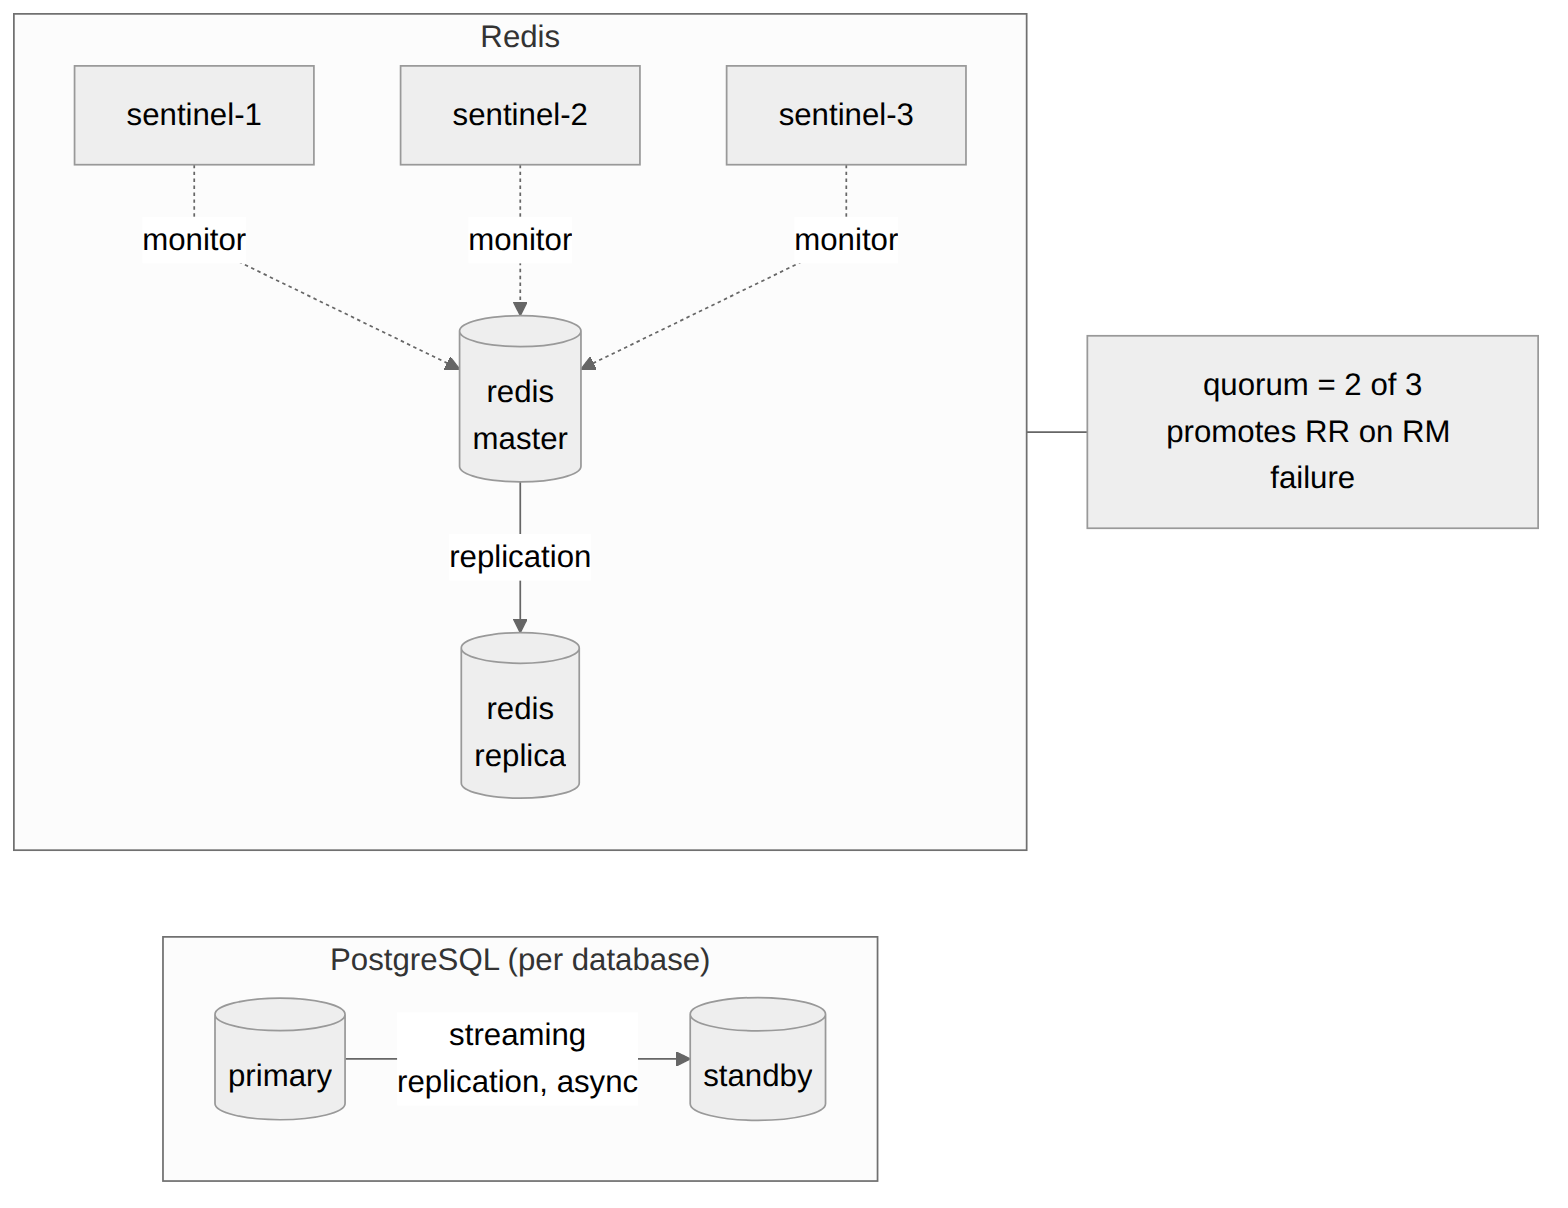
\includegraphics[width=0.85\textwidth]{figures/replication-ha.png}
\caption{PostgreSQL streaming replication and the Redis Sentinel quorum.}
\label{fig:replication-ha}
\end{figure}

\subsubsection{Fail-Open Cache and Rate Limiter}\label{fault-tolerance-fail-open}

Both the gateway's proxy cache and its distributed rate limiter are designed to \textbf{fail
open}: if a Redis/Sentinel read throws, the gateway logs a warning and falls through to the
upstream fetch (for the cache) or allows the request through anyway (for the rate limiter),
rather than failing the whole request. This was not the original behaviour of the rate limiter:
an internal audit of the system found that it originally had no such fallback and would have
taken down \emph{all} gateway traffic on a Redis blip; this was fixed before this report was
written. Cache failure falls back to an upstream request, not to a guaranteed durable stale copy.
If that request also fails, an error is returned. Repository persistence follows a different
policy: invalid batches roll back and propagate failure. Best-effort HTTP-side persistence may
log that failure separately; it does not turn a partially committed batch into a successful one.

\subsubsection{Resumable Imports on Restart}\label{fault-tolerance-backfill}

The durable jobs and checksum ledger in \cref{modelling-backfill-gate} are the restart checkpoint.
Completed files are skipped, incomplete work remains pending, and failed providers yield through
a retry delay. A bounded file batch avoids keeping the worker on one large import indefinitely.
This provides practical resumability with transactional deduplication, not an exactly-once
processing guarantee for an arbitrarily replicated ingestion service.

\subsubsection{Database Connection Retry and Startup Ordering}\label{fault-tolerance-retry}

The ingestor retries its initial database connection with capped linear backoff. HTTP services
initialize persistence on a best-effort basis and expose dependency readiness separately from
liveness. Their HikariCP acquisition and validation deadlines keep a failed dependency from
blocking indefinitely; pool resources close on application shutdown.

Compose currently uses short-form dependency lists. These order container starts but do not wait
for database readiness. Some services define health checks, yet those checks are not automatically
startup gates; an explicit \texttt{service\_healthy} condition would be required for that behavior
\citep{docker2026startup}. Startup races are therefore an operational limit, mitigated by the
worker's retry loop and observable through readiness, not eliminated by orchestration.

\subsection{Availability}\label{availability}

\subsubsection{Caching}\label{availability-caching}

The gateway caches upstream responses (market prices, market history, news, news history) keyed
by the request's distinguishing parameters, with a short TTL. When Redis is configured, this
cache is shared across every gateway replica, which is what actually makes running more than one
replica worthwhile, since otherwise each replica would cache (and warm its cache) independently.
When Redis is not configured, the gateway falls back to a bounded in-process cache, which is
correct for a single instance but would silently stop being a \emph{shared} cache across multiple
replicas. Range-history and timestamped-history proxy routes bypass this cache so newly imported
coverage can be observed without a stale gateway entry. News-service keys have their own
namespace, preventing collision with gateway response envelopes.

\subsubsection{Load Balancing}\label{availability-load-balancing}

An nginx instance (\texttt{gateway-lb}) fronts however many \texttt{gateway} containers are
running. It uses a variable upstream and Docker's DNS resolver with a short validity period,
allowing discovery to refresh when the gateway set changes. This is paired with the Redis-backed distributed rate limiter
(\cref{fault-tolerance}): load balancing across replicas would otherwise multiply the effective
rate limit by the number of replicas, since Ktor's own built-in rate limiter keeps its counters
in-process.

\begin{figure}
\centering
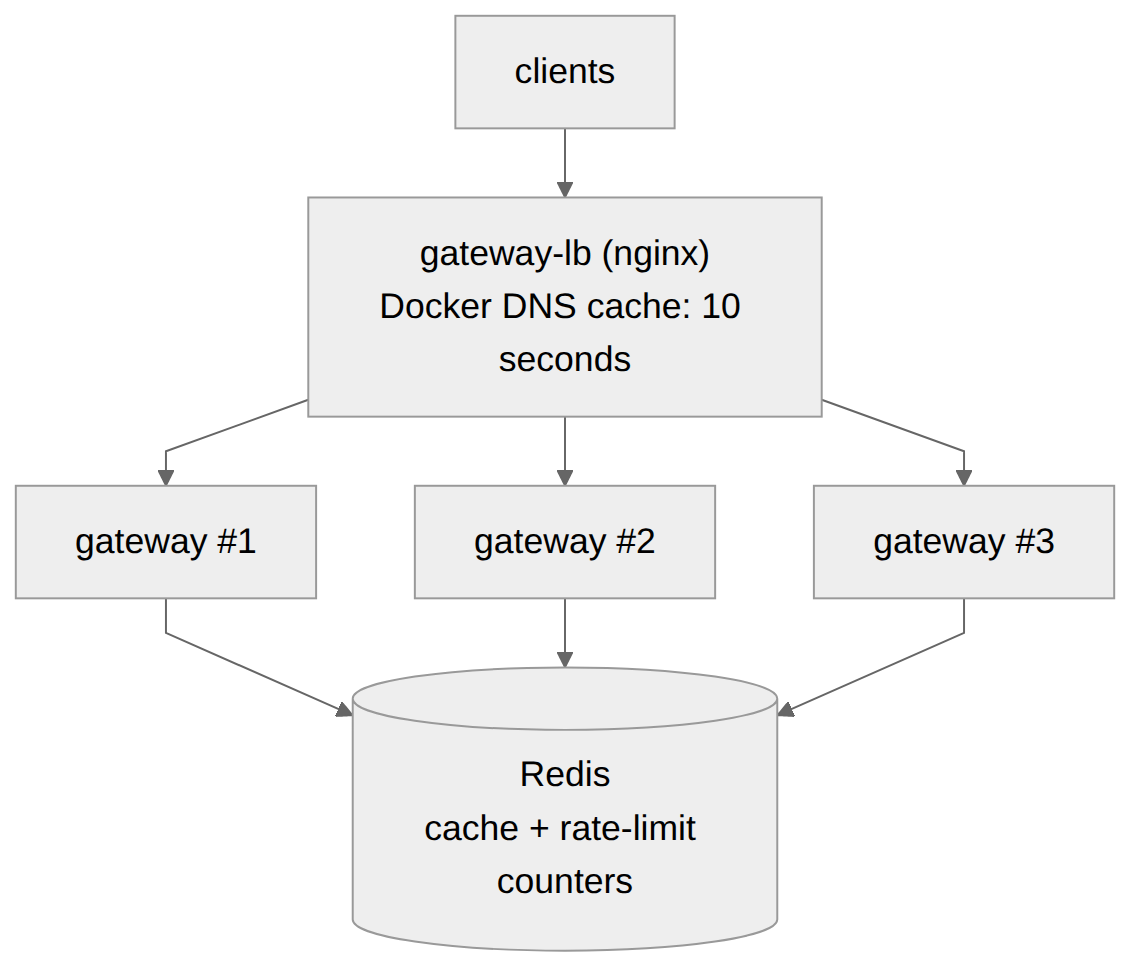
\includegraphics[width=0.7\textwidth]{figures/load-balancing.png}
\caption{Gateway replicas behind \texttt{gateway-lb}, sharing state only via Redis.}
\label{fig:load-balancing}
\end{figure}

\subsubsection{Network Partition Behaviour}\label{availability-partitions}

Two different partition scenarios are handled differently by design. A partition that isolates a
PostgreSQL standby from its primary simply stalls replication until it heals, since the primary
keeps serving reads and writes unaffected, given that replication here is asynchronous and
one-way. A partition that isolates a minority of the Redis Sentinel quorum (at most one of three
Sentinels, given quorum size 2) does not block failover decisions, since the remaining two
Sentinels still form a quorum; a partition that isolated a \emph{majority} of Sentinels would
correctly block failover rather than risk a split-brain promotion, at the cost of not being able
to fail over at all until it heals. That is a standard, intentional trade-off of quorum-based
systems~\citep{redis2024sentinel}, not a flaw specific to this deployment.

\subsection{Security}\label{security}

\subsubsection{Current State}\label{security-current}

The public HTTP API has no account authentication, JWT validation, or role-based authorization.
The Keycloak/OIDC design below is a proposal: there is no Keycloak service or client login flow.
Internal database credentials and infrastructure configuration are still security-sensitive;
an anonymous product does not make every component or operational datum public.

Implemented hardening includes the following controls:
\begin{itemize}
  \item Published development ports bind to loopback. Grafana and pgAdmin require the optional
  admin profile; database and admin credential placeholders must be replaced before exposure.
  \item The private nginx ingress overwrites forwarding headers. The gateway trusts this
  boundary, shares Redis-backed client budgets, and exempts liveness/readiness/metrics probes.
  \item HTTP requests and connection acquisition have deadlines. Client-visible failures use safe
  envelopes rather than raw upstream exception details; invalid range/category input is rejected.
  \item Runtime service images use a non-root UID. Docker context exclusions keep credentials,
  Git metadata, generated output, and report files out of application images.
  \item Archive hosts and paths are constrained; downloads and expanded ZIP data are bounded,
  XML external entities are disabled, checksums are required, and no archive path is extracted.
  \item Dependency versions receive targeted security upgrades, with weekly Dependabot proposals
  and a PR dependency-review check. This is not a claim that dependency risks are eliminated.
\end{itemize}

Redis rate limiting deliberately fails open on backend errors. Public TLS termination, complete
secret distribution, user identity, and authorization for future private/write APIs remain outside
the current local development topology.

\subsubsection{Proposed Identity Design (Not Implemented)}\label{security-identity}

Rather than have each service manage credentials independently, Orbital would introduce a
dedicated identity provider, Keycloak, as a new infrastructural component alongside the existing
Postgres/Redis/Prometheus stack (\cref{infrastructure}). Keycloak would own a single realm for
the project and issue signed JSON Web Tokens (JWTs,~\citep{jones2015jwt}) after an OpenID Connect
(OIDC)~\citep{sakimura2014oidc} Authorization Code flow with PKCE, the flow recommended for
public clients that cannot keep a client secret, which matches \texttt{orbital-app}'s nature as a
Kotlin Multiplatform client distributed as a desktop binary and a static web build, neither of
which can safely embed one.

Centralizing identity this way is a natural fit for Orbital's existing architecture rather than a
bolt-on. The client already talks exclusively to the gateway (\cref{architecture}), so the
gateway would remain the single trust boundary where tokens are validated, exactly as it is
already the single point where caching and rate limiting are enforced. Validation itself would be
stateless: the gateway would install an \texttt{Authentication} plugin with a JWT provider,
fetching Keycloak's signing keys from its JWKS endpoint and caching them locally, refreshed on a
TTL, the same pattern already used elsewhere in the system for distributed state
(\cref{availability}). Because JWT validation needs no round-trip to Keycloak nor a shared session
store, it composes cleanly with the horizontal-scalability work already done on the gateway: any
number of gateway replicas behind the load balancer could validate tokens independently, with no
new shared state and no new single point of failure introduced by the validation step itself.

\begin{figure}
\centering
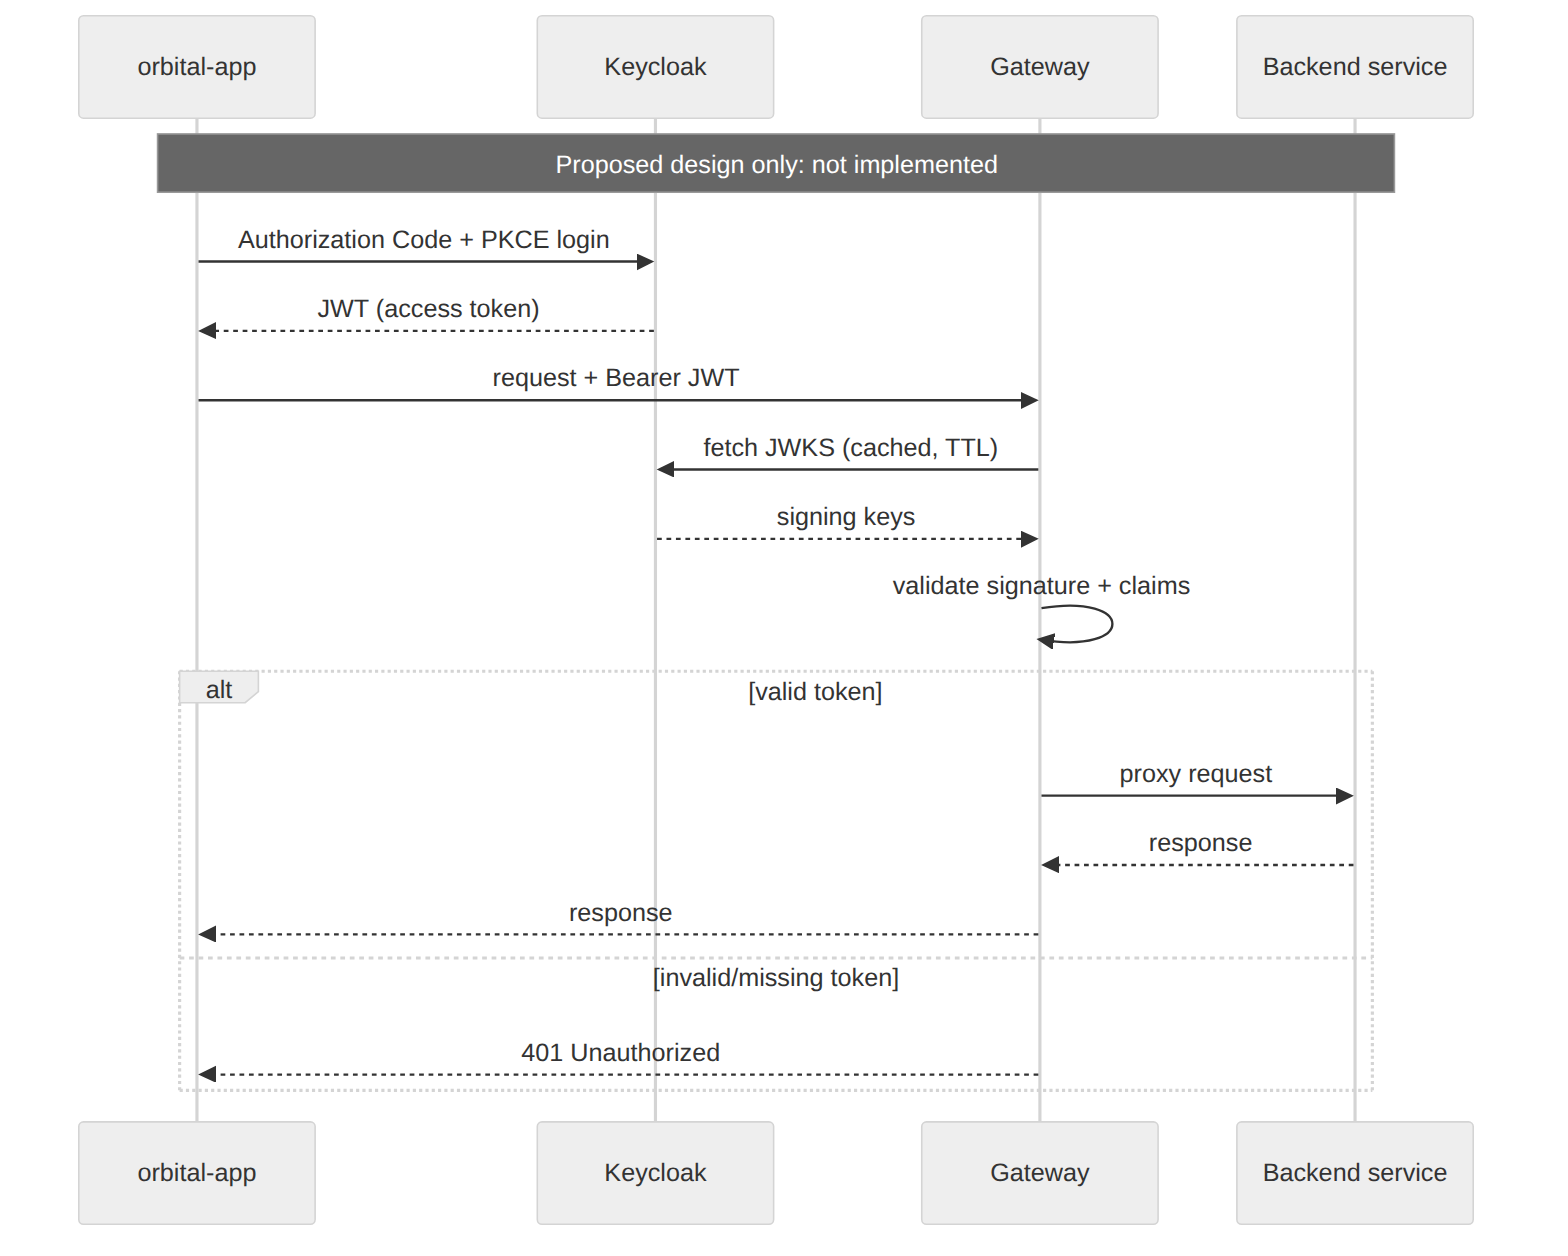
\includegraphics[width=0.85\textwidth]{figures/keycloak-auth-flow.png}
\caption{Proposed OIDC/JWT authentication flow (not implemented).}
\label{fig:keycloak-auth-flow}
\end{figure}

\subsubsection{Proposed Authorization Model (Not Implemented)}\label{security-authz}

Authorization would be expressed through realm roles embedded as claims in the JWT (e.g.\
\texttt{user}, \texttt{premium}, \texttt{admin}), rather than through a separate access-control
service. Given Orbital's current product shape, the most natural use of these roles would not be
gatekeeping the existing read endpoints (which are deliberately public) but tiering them:
authenticated requests could be granted a materially higher entry in the distributed rate limiter
(\cref{availability}) than anonymous ones, and any future write-capable or administrative endpoint
(e.g.\ forcing a cache invalidation, or re-triggering a historical backfill in the market
ingestion worker) would require the \texttt{admin} role. This keeps the public-aggregator
character of the product intact while still giving the system a real authorization story.

\subsubsection{Keycloak's Own Fault Tolerance (Not Implemented)}\label{security-keycloak-ha}

Keycloak itself would need the same fault-tolerance treatment already applied to Orbital's other
stateful components (\cref{fault-tolerance}): it requires its own relational database for realm
and user state, and running it as a single instance would reintroduce exactly the kind of single
point of failure that the Postgres and Redis replication work in this project was meant to
eliminate. A production-oriented deployment would therefore either run Keycloak against one of the
already-replicated Postgres instances, on a dedicated schema, or, more robustly, run Keycloak
itself in clustered mode across two or more nodes.

\section{Implementation}\label{implementation}

\subsection{Network Protocols and Data Representation}\label{impl-network}


Client/gateway/service APIs and CoinGecko responses use HTTP/JSON. Success responses carry a
\texttt{data} envelope; failures use structured status/message envelopes. Historical timestamps
are normalized to Unix seconds and displayed in UTC. Internal PostgreSQL and Redis traffic uses
their native client protocols.

Binance imports instead use HTTPS listing XML, checksum text, and compressed ZIP/CSV files.
The worker verifies and parses those representations before storing typed records. There is no
external message broker, server-push market stream, or project-specific binary RPC protocol.

\subsection{Data Persistence and Querying}\label{impl-persistence}

Exposed manages tables and transactional repository operations. Historical range selection also
uses prepared JDBC SQL with \path|ROW_NUMBER| partitioning and time buckets. Table/column names
come from fixed source choices, while coin IDs and numeric bounds are bound as statement
parameters. It would therefore be inaccurate to describe every query as Exposed DSL or to base
SQL-injection protection solely on the ORM.

Schema setup uses \texttt{createMissingTablesAndColumns} for additive tables, columns, and
indexes. Tests cover adding the coin/time index to an older schema. Compatibility endpoints and
legacy rows are retained; this is not a general versioned migration or destructive cleanup system.
New range queries sample full selected windows; legacy history reads keep their latest-500 bound.

\subsection{Authentication and Authorization}\label{impl-auth}

As detailed in \cref{security}, public API callers have no account authentication or
role-based authorization. Database connections use configured credentials, but the application
has no OAuth/JWT validation or RBAC/ABAC policy. A concrete,
unimplemented design for closing this gap (OIDC via Keycloak, JWTs validated at the gateway, role
claims driving a tiered rate limit) is proposed in \cref{security} and listed again in
\cref{future-works}.

\subsection{Frontend Implementation}\label{impl-frontend}

The common Compose UI is shared by desktop JVM and WebAssembly browser targets. Stable coin keys
preserve expansion state; refresh mutexes serialize overlapping requests. Previous content remains
visible after refresh failures, with a stale-data notice and retry action. HTTP clients close when
their owning composition ends. Search fields are labelled, empty lists are explained, and article
buttons open HTTPS links. Synthetic news is identified in the UI.

The full \texttt{MarketApiClient} loads \texttt{HistorySeries} through the range endpoint.
Changing source/range/viewport cancels obsolete work; incomplete imports are polled periodically.
24H and 7D are fixed durations, 1M uses 30 days, and 1Y uses 365 days. All available spans loaded
history and requests the remaining daily archive. Both platforms expose zoom buttons; the browser
also observes pan/wheel changes and desktop supports wheel zoom. Finer requests cannot create
unpublished provider data or promise resolution unavailable under the public plan.

Browser charts use the bundled Lightweight Charts library. Desktop charts use native Canvas.
Both preserve real timestamps and split line segments across reported gaps. The old timestamped
adapter remains available, while the backend-free demo uses explicitly relative seven-day samples
and does not offer persistent archive controls. Small USD values retain additional decimals;
values below the supported display precision receive an explicit threshold label.

\subsection{Containerization and Orchestration}\label{impl-containers}

Every backend component is containerized with Docker. Each Ktor service (gateway, market-service,
news-service) has a multi-stage \texttt{Dockerfile}: a build stage using
\texttt{eclipse-temurin:21-jdk} to produce a fat JAR via Gradle's \texttt{shadowJar}, and a
runtime stage using the much smaller \texttt{eclipse-temurin:21-jre}. \texttt{market-ingestor}
reuses market-service's own build output via a separate \texttt{Dockerfile.ingestor} that differs
only in its entrypoint (\texttt{com.orbital.market.MarketIngestorKt} instead of the HTTP server's
\texttt{main}), rather than duplicating the build. One \texttt{docker-compose.yml} defines the
backend system on one bridge network, with
environment variables for service URLs, credentials, and feature toggles (such as
\path|REDIS_SENTINEL_HOSTS|) injected per service. Health checks observe service status;
short-form dependencies do not enforce readiness (\cref{fault-tolerance-retry}). Runtime images
use UID 10001 and JVM limits use \path|JAVA_TOOL_OPTIONS|; build context exclusions and
Gradle cache mounts separate source, credentials, and generated artifacts. \Cref{deployment} gives the full per-service breakdown.

\subsection{Technological Details}\label{technological-details}

\begin{itemize}
  \item \textbf{Kotlin 2.3.21} for application code; Gradle wrapper 8.14.
  \item \textbf{Ktor}~\citep{ktor2024docs}: backend 2.3.13 and client 3.5.2 remain separate
  because WebAssembly support has different requirements. Netty is constrained to 4.1.140.Final.
  \item \textbf{Compose Multiplatform}: the \texttt{orbital-app} client, JVM desktop and
  \texttt{wasmJs} web from one codebase (Compose 1.12.0, Material3 1.9.0).
  \item \textbf{Exposed} / \textbf{HikariCP} against \textbf{PostgreSQL
  15}~\citep{postgresql2024docs}: all persistence; \textbf{H2} (PostgreSQL-compatibility mode)
  supports fast tests, with a separate real-PostgreSQL repository CI job. PostgreSQL JDBC is
  42.7.14 and Logback is 1.6.6 in the reviewed snapshot.
  \item \textbf{Jedis}, behind an internal abstraction supporting either a plain
  \texttt{JedisPool} or a Sentinel-aware \texttt{JedisSentinelPool}~\citep{redis2024sentinel}.
  \item \textbf{nginx}: \texttt{gateway-lb}'s load balancer.
  \item \textbf{Prometheus} and \textbf{Grafana}: metrics collection and visualization, via a
  Micrometer-backed \texttt{/metrics} endpoint on each HTTP service.
  \item \textbf{Docker Compose}~\citep{docker2024compose}: the sole deployment/orchestration
  mechanism.
  \item \textbf{Gradle} (multi-module), with \textbf{detekt} and \textbf{ktfmt}/\textbf{spotless}
  enforced in CI, and \textbf{GitHub Actions} + \textbf{release-please} automating testing,
  Docker image builds, and versioned releases from Conventional Commit history.
\end{itemize}

\section{Validation}\label{validation}

\subsection{Automatic Testing}\label{automatic-testing}

\subsubsection{Test Infrastructure}\label{testing-infrastructure}

The full validation command is \texttt{./gradlew check}, covering backend, shared libraries,
desktop, browser tests, and read-only detekt/formatting checks. Formatting is a separate explicit
operation. Ktor \texttt{testApplication} and \texttt{MockEngine} isolate HTTP behavior; repository
tests can use H2 or a disposable PostgreSQL instance. Fake Redis operations cover deterministic
rate-limit decisions without pretending to validate real quorum timing.

A separate CI job starts PostgreSQL 15 and reruns repository tests with build-cache reuse disabled.
Each test creates an isolated schema. The client suite includes Compose desktop state/interaction
checks and common tests also executed in a headless browser. This provides automated client
coverage; manual screen-reader conformance and an exhaustive native-window walkthrough are not
claimed.

\subsubsection{Recorded Coverage}\label{testing-coverage}

The archived implementation validation recorded the following executions on 13 November 2026.
Common tests run on multiple targets, so this is an execution count rather than a claim of 83
unique test methods. This report update does not relabel those results as a fresh run.

\begin{center}
\begin{tabular}{lrr}
\toprule
Module & Executions & Failures \\
\midrule
Market service & 35 & 0 \\
Gateway & 15 & 0 \\
News service & 10 & 0 \\
Core library & 1 & 0 \\
Models library & 2 & 0 \\
Client: desktop/browser & 20 & 0 \\
\midrule
Total & 83 & 0 \\
\bottomrule
\end{tabular}
\end{center}

\paragraph{Market history and integrity (FR2, FR7).} Tests cover ascending legacy history,
atomic rollback, deterministic deduplication, schema upgrades, and the separation of live
observations from completion metadata. Archive tests cover millisecond/microsecond conversion,
closing timestamps/prices, invalid values and paths, checksum failure/success, safe ZIP reading,
listing pagination, and monthly/daily selection. Range tests cover observations older than the
former 500-point cap, separate USD/USDT series, untracked/inactive assets, gaps, finer windows,
invalid bounds, file-ledger idempotency, and delayed-job fairness.

\paragraph{News and gateway behavior (FR3, FR4, NFR1--NFR5).} Repository tests verify rollback
and history ordering/filtering; HTTP tests cover response contracts and categories. Gateway tests
cover short-TTL cache hits, cache failure, client-key isolation, quota exhaustion, fail-open
behavior, forwarding trust, CORS, and liveness after the public request budget is exhausted.

\paragraph{Client interaction (FR5, FR6).} Tests cover search state across visibility changes,
initial failure versus stale content, sub-cent formatting, history request parameters and coverage
decoding, source/range/zoom selection, cancellation of obsolete requests, and unavailable Binance
selection for unlisted assets. Browser fixtures verify range changes, real chart wheel callbacks,
source switching, segmented gaps, and a 390-pixel mobile layout without horizontal overflow.
Synthetic fixture screenshots are not evidence of live historical market values.

\par\medskip\noindent\begin{minipage}{\linewidth}
\subsubsection{How to Run}\label{testing-how-to-run}

\par\medskip\noindent\begin{minipage}{\linewidth}
\begin{verbatim}
./gradlew check
./gradlew ktfmtFormat     # explicit source formatting, not validation
./gradlew --no-build-cache --rerun-tasks \
  :market-service:test :news-service:test --tests '*RepositoryTest'
\end{verbatim}
\end{minipage}\par\medskip
\end{minipage}\par\medskip

The repository run needs \path|TEST_POSTGRES_URL|, \path|TEST_DB_USER|, and
\path|TEST_DB_PASSWORD| configured for a disposable database. Browser checks need Chromium;
\path|CHROME_BIN| selects a non-default installation. Reports are written beneath each module's
\path|build/reports/tests/| directory.

\subsection{Runtime and Acceptance Evidence}\label{acceptance-test}

Recorded evidence is retained with the repository in the review documentation and archives:
\path|docs/review/REMEDIATION.md|, \path|docs/review/HISTORY.md|, and
\path|docs/review/artifacts/|. Those records distinguish synthetic fixtures, real-provider checks,
and manual infrastructure scenarios.

\begin{itemize}
  \item \textbf{Database behavior:} uncached real-PostgreSQL tests exercised transactional
  failure, timestamped history, and schema setup/upgrades. Earlier replication inspection on the
  market primary observed an actively streaming standby and matching WAL positions at that time.
  \item \textbf{Redis and gateway failure paths:} recorded checks covered replica promotion,
  restart of all three Sentinels while preserving the promoted master, health after quota
  exhaustion, forwarded-identity handling, readiness degradation on database loss, safe upstream
  errors, and the non-root runtime user. These are bounded scenarios, not a sustained-load SLA.
  \item \textbf{Real archive import:} Binance BTCUSDT August 2017 data passed SHA-256 validation;
  all 15 daily candles were stored in an isolated PostgreSQL database. Re-importing did not add
  duplicate candles. The earliest closing time was 17 August 2017 at 23:59:59 UTC. This verifies
  one real import path, not every coin/file in the provider archive.
  \item \textbf{Interactive preview:} the subsequent local app run returned 20 tracked coins and
  imported Bitcoin coverage back to August 2017. It was stopped without removing database data.
  \item \textbf{CI and release integration:} the full PR suite, Commitlint, and Dependency Review
  passed in the recorded remote runs. A separate push job encountered Maven Central HTTP 429
  during dependency download before tests started; it is an infrastructure failure, not a failed
  PostgreSQL assertion. One immutable legacy commit receives an exact-SHA leading-space
  normalization in CI; all other commit messages remain strictly checked.
\end{itemize}

Sustained multi-replica load, automated PostgreSQL promotion, production TLS/secrets management,
complete provider coverage, manual accessibility conformance, and native installers remain
outside the validated scope. No result above implies those outstanding properties.

\section{Deployment}\label{deployment}

\subsection{Prerequisites}\label{deployment-prerequisites}

The following software must be installed on the host machine:
\begin{itemize}
  \item \textbf{Docker} with Docker Compose v2.
  \item \textbf{JDK 21} for native application/Gradle commands; containers supply their own JDK/JRE.
  \item \textbf{Chromium/Chrome} for browser tests. Node.js 22 and npm are needed for the
  repository Commitlint/Husky tooling; the WebAssembly build manages its own JavaScript toolchain.
  \item A free CoinGecko Demo key for authenticated public-plan historical requests. Binance
  archive downloads require no API key; provider quotas and dataset terms still apply.
\end{itemize}

\subsection{Installation from Scratch}\label{deployment-installation}

\begin{enumerate}
  \item \textbf{Clone the repository and configure environment variables:}
\par\medskip\noindent\begin{minipage}{\linewidth}
\begin{verbatim}
git clone <repository-url>
cd orbital
cp .env.example .env
\end{verbatim}
\end{minipage}\par\medskip
  Every variable in \texttt{.env} has a safe, documented default for local development; only
  credential-related variables (\path|POSTGRES_MARKET_PASSWORD|,
  \path|POSTGRES_NEWS_PASSWORD|, \path|POSTGRES_REPLICATION_PASSWORD|,
  \path|GRAFANA_ADMIN_PASSWORD|, \path|PGADMIN_ADMIN_PASSWORD|) must be overridden before
  any deployment reachable over a real network. These replaced plaintext defaults that
  \texttt{docker-compose.yml} previously hardcoded directly, an issue identified and fixed during
  this project's own security audit.

  Set \path|COINGECKO_DEMO_API_KEY| for public-plan history and retain the default
  \texttt{INGEST\_INTERVAL\_MS=900000} unless a different collection cadence is intended.

  \item \textbf{Build and start the backend:}
\par\medskip\noindent\begin{minipage}{\linewidth}
\begin{verbatim}
make up        # equivalent to: docker compose up --build -d
\end{verbatim}
\end{minipage}\par\medskip
  Schema setup is additive through Exposed (\cref{impl-persistence}); the ingestor retries until
  its database is available. Inspect \path|/ready| rather than treating container start or
  \path|/health| as proof that every dependency is usable. Historical imports fill progressively.
  Admin consoles are optional: \texttt{docker compose --profile admin up -d}. Published ports
  bind to \texttt{127.0.0.1}.

  \item \textbf{Verify deployment:}
\par\medskip\noindent\begin{minipage}{\linewidth}
\begin{verbatim}
curl localhost:8080/health
curl localhost:8080/ready
curl localhost:8080/api/v1/market/prices
curl localhost:8080/api/v1/news
\end{verbatim}
\end{minipage}\par\medskip
  Expected outcome: liveness from the first call, dependency readiness from the second, live
  CoinGecko prices from the third, and the synthetic crypto feed from the fourth. Dependency or
  provider failures can return a safe error instead; inspect readiness and logs before proceeding.
\end{enumerate}

\subsubsection{Docker Compose Services}\label{deployment-services}

\texttt{docker-compose.yml} defines the following 17 services:

\begin{itemize}
  \item \textbf{gateway:} The API gateway. Proxies, caches, and rate-limits requests to the two
  backend services. No fixed published port: \texttt{gateway-lb} is the host's actual entry
  point, so that it can be scaled to multiple replicas.
  \item \textbf{gateway-lb:} nginx, published on host port \texttt{8080}. Load-balances across
  however many \texttt{gateway} replicas are running.
  \item \textbf{market-service:} The market-data REST API, published on port \texttt{8081}.
  Depends on \texttt{postgres-market} and \texttt{redis}.
  \item \textbf{market-ingestor:} The standalone ingestion worker (FR7). No published port.
  Depends on \texttt{postgres-market}.
  \item \textbf{news-service:} The news REST API, published on port \texttt{8082}. Depends on
  \texttt{postgres-news} and the Redis/Sentinel cluster.
  \item \textbf{postgres-market / postgres-news:} The two independent PostgreSQL 15 primaries,
  published on loopback ports \texttt{5432}/\texttt{5433}. Their \texttt{pg\_isready} health
  checks do not gate short-form Compose dependencies.
  \item \textbf{postgres-market-replica / postgres-news-replica:} Streaming-replication standbys
  of the two primaries, cloned via \texttt{pg\_basebackup} on first start.
  \item \textbf{redis:} The Redis cache primary, published on port \texttt{6379}.
  \item \textbf{redis-replica:} A replica of \texttt{redis}, for Sentinel to promote on failover.
  \item \textbf{redis-sentinel-1/2/3:} The three-node Sentinel quorum (quorum size 2) monitoring
  \texttt{redis}/\texttt{redis-replica}.
  \item \textbf{prometheus / grafana:} Metrics collection (port \texttt{9090}) and visualization
  (port \texttt{3000}, admin profile), with a provisioned ``Orbital Overview'' dashboard.
  \item \textbf{pgadmin:} An optional administration UI (loopback port \texttt{5050}, admin
  profile) for both databases.
\end{itemize}

All services share a single Docker bridge network (\texttt{orbital-net}), enabling inter-container
communication by service name (\cref{infrastructure}).

\subsubsection{Startup Ordering and Health Checks}\label{deployment-health}

Compose dependency lists start dependencies before their consumers, but the current short-form
configuration does not wait for \texttt{service\_healthy}. Readiness and the ingestor's retry loop
are therefore important; startup ordering alone cannot establish availability
\citep{docker2026startup}. Operators should inspect service logs and readiness after boot.

Redis/Sentinel runtime state is stored in separate writable volumes instead of rewriting checked-in
configuration. Numeric topology addresses survive ordinary container/Sentinel restarts on the same
network. If the whole Docker network is recreated, the disposable Redis/Sentinel topology must be
reinitialized coherently. PostgreSQL volumes must not be included in that cache reset.
Use \texttt{docker compose stop} to stop without removing containers or data; ordinary
\texttt{docker compose down} preserves named volumes. The clean target that removes volumes is
destructive and is not the routine shutdown procedure.

\subsection{Rebuilding Individual Services}\label{deployment-rebuild}

A single service can be rebuilt and restarted without affecting the others:
\par\medskip\noindent\begin{minipage}{\linewidth}
\begin{verbatim}
docker compose up --build gateway
\end{verbatim}
\end{minipage}\par\medskip

\subsection{Schema Management}\label{deployment-schema}

Unlike a Liquibase/Flyway-based migration tool, Orbital applies schema changes automatically at
each service's startup, via Exposed's \texttt{createMissingTablesAndColumns}
(\cref{impl-persistence}); there is no separate ``run the migrations'' command, and none is
needed: starting (or restarting) \texttt{market-service} or \texttt{news-service} is itself the
migration step. This was a deliberate simplicity trade-off for a project of this size, with the
trade-off made explicit rather than assumed: \cref{automatic-testing} reports an automated test
that specifically verifies this mechanism retroactively adds a newly-introduced index to an
already-existing table, since that guarantee cannot simply be assumed of every Exposed version.

\par\medskip\noindent\begin{minipage}{\linewidth}
\section{User Guide}\label{user-guide}

The backend can be inspected through HTTP. The following examples keep compatibility reads and
range-aware reads distinct:

\par\medskip\noindent\begin{minipage}{\linewidth}
\begin{verbatim}
curl localhost:8080/api/v1/market/prices
curl 'localhost:8080/api/v1/market/history-range/bitcoin?range=all'
curl 'localhost:8080/api/v1/market/history-range/bitcoin' \
  --get --data 'range=24h' --data 'source=binance'
curl localhost:8080/api/v1/market/history-points/bitcoin
curl localhost:8080/api/v1/market/history/bitcoin
curl 'localhost:8080/api/v1/news?category=crypto'
\end{verbatim}
\end{minipage}\par\medskip
\end{minipage}\par\medskip

The connected client is started after the backend:
\par\medskip\noindent\begin{minipage}{\linewidth}
\begin{verbatim}
./gradlew :orbital-app:run
./gradlew :orbital-app:wasmJsBrowserDevelopmentRun
\end{verbatim}
\end{minipage}\par\medskip

Expand a coin to select 24H, 7D, 1M, 1Y, or All available. Choose Binance USDT or CoinGecko USD;
Binance selection is disabled without a verified pair. Use zoom controls, browser pan/wheel, or
desktop wheel input to request a narrower window. Coverage labels show loaded dates, displayed
resolution, import progress, and gaps. A loading or empty view is not evidence that the coin has
no earlier history: work may still be queued or outside the provider's coverage. Keep the ingestor
running while coverage fills.

The news tab contains clearly labelled synthetic crypto articles, search/category filters, and
HTTPS article actions. Unsupported populated categories are not implied by the interface. Both
views refresh periodically, and a failed refresh can retain stale content with a retry notice.

The release-hosted market-only demo at \url{https://loch3f.github.io/orbital/} calls CoinGecko
directly. It has no news tab, persistent server-side archive, or full historical range controls.
Its seven-day sparkline is a relative trend, not the complete exchange history.

\paragraph{CI and release workflow.} Feature work is reviewed into \texttt{develop}; promotion
into protected \texttt{main} uses a pull request and passing checks. Merge commits preserve shared
ancestry for these long-running branches. Release Please subsequently proposes version/changelog
updates. After a release or main-only hotfix, synchronize main back into develop, keeping release
metadata and security/build changes together when resolving conflicts. Dependabot configuration
is evaluated on the default branch; its weekly proposals still require review, tests, and merging.
The Docker update entry currently covers the gateway directory only. This is not a promise that
all container images are automatically updated.

\section{Self-evaluation}\label{self-evaluation}

\subsection{Aldo Visconti}\label{self-evaluation-aldo}

This is a single-author project, so one section follows rather than one per group member.

\paragraph{Role.} As the sole developer of this project, I was responsible for every aspect of
the system: requirements elicitation, architectural design, backend implementation across the
gateway and both backend services, the market-ingestion worker, the client application, the
infrastructure work described in \cref{fault-tolerance} and \cref{availability}, and both
automated and manual testing.

\paragraph{Strengths.} Separating collection from API traffic removes a major source of
inconsistent history growth. Durable import jobs and a checksum ledger make progress visible and
recoverable without treating a single live price as complete backfill. Source-labelled USD/USDT
series preserve provider differences instead of hiding them in one chart. Atomic rollback,
deterministic identities, and tests against PostgreSQL strengthen the meaning of persisted data.

The hardening work also made operational behavior explicit: forwarding trust, probe exemptions,
readiness, safe errors, resource deadlines, pool cleanup, non-root images, and bounded archive
parsing each address a concrete failure or abuse path. Recorded runtime checks complement unit
and UI tests without being presented as a universal production guarantee. Keeping domain modules
and client adapters separate supported these changes without introducing a message broker or a
second client codebase.

\paragraph{Weaknesses and Limitations.} This remains a single-author academic project with an
internal, assisted review rather than an independent security assessment. Realistic sustained
multi-replica load, complete archive coverage for every tracked coin, and manual accessibility
validation remain open. The single-worker queue lacks distributed leasing; asynchronous replicas
can lag; PostgreSQL promotion is manual; provider quotas can interrupt collection. Public API
reads remain anonymous and the production TLS/secrets/distribution story is incomplete.
The public demo deliberately exposes less functionality than the connected application.
These boundaries are part of the evaluation rather than completed requirements disguised as
future work.

\section{Future works}\label{future-works}

\paragraph{Automatic database failover.} Both PostgreSQL standbys (\cref{fault-tolerance}) give
Orbital a replica of each database, subject to replication lag, but nothing promotes a standby to primary
or repoints a backend service's \path|DB_URL| automatically if a primary fails. That is
normally the job of a dedicated tool such as Patroni or repmgr, deliberately left out of this
project as a separate, larger piece of work rather than attempted partially.

\paragraph{Verifying scalability under real load.} The nginx load balancer and the distributed
rate limiter were both designed specifically to make running multiple \texttt{gateway} replicas
safe (NFR3), and both compile and pass their own unit/integration tests, but neither has actually
been exercised against several \emph{scaled} replicas under concurrent load, e.g.\
\texttt{docker compose up --scale gateway=3} followed by sustained traffic, checking that the
rate limit really is enforced once, globally, rather than once per replica. This is the natural
next step beyond the manual verification already performed (\cref{acceptance-test}).

\paragraph{Synchronous replication.} \Cref{cap-theorem-position} discusses the asynchronous replication trade-off.
A future iteration could make replication mode configurable, accepting additional write latency
and reduced write availability when a required standby is unreachable. Durability would still
depend on the acknowledgement policy and promoting a sufficiently synchronized standby.

\paragraph{Broader client and import validation.} Desktop, common, and browser tests now exist
(\cref{automatic-testing}). Further work should add manual screen-reader testing, native-window
walkthroughs, larger provider fixtures, longer import interruption scenarios, and sustained
concurrent multi-replica load. Existing automated checks do not replace those evaluations.

\paragraph{Real news integration.} News-service currently serves a synthetic feed without
external requests rather than using a configured NewsAPI subscription (\cref{ds-features}'s economy discussion); wiring up the real
integration behind the same interface it already exposes (\texttt{NewsApiClient}) would be a
contained change once the cost trade-off is revisited.

\paragraph{Authentication and authorization.} As discussed in \cref{security}, Orbital has no
authentication or authorization layer today. The concrete next step is the Keycloak-based design
proposed there: a dedicated identity-provider service issuing OIDC/JWT tokens, validated
statelessly at the gateway, with realm-role claims driving a tiered rate limit between
authenticated and anonymous traffic, and gating any future write-capable endpoint. This remains
future work rather than a completed feature.

\bibliographystyle{plain}
\bibliography{references}

\end{document}
